\chapter{Spawning and catching}
\label{chap:spawn}
\textbf{FIXME}

\section{Wild spawns}
\label{sec:spawns}
\textbf{FIXME}

\section{Catching}
\label{sec:catch}
\textbf{FIXME}

\subsection{Berries}
Berries can enhance the catching process (\autoref{table:berries}).
Only one Berry can be applied to a Pokémon at a time.
The Berry is consumed upon use, but persists on the Pokémon across Pokéballs
  and even encounters (i.e., you can leave the encounter, and if you return,
  the Berry will still be applied).
If the Pokémon escapes a Pokéball, however, any applied Berry is gone forever.
A new Berry can be used in this case.

\begin{table}[ht]
\begin{center}
\begin{tabular}{lll}
Berry & Effect & How to acquire \\
\Midrule\\
Razz 
\includegraphics[width=1em]{images/razz.png} & & \\
Nanab 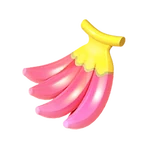
\includegraphics[width=1em]{images/nanab.png} & & \\
Pinap 
\includegraphics[width=1em]{images/pinap.png} & & \\
Silver Pinap 
\includegraphics[width=1em]{images/silverpinap.png} & &\\
Golden Razz 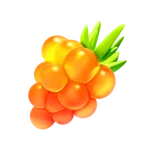
\includegraphics[width=1em]{images/goldenrazz.png} & & \\
\end{tabular}
\end{center}
\caption{Berries and their uses}
\label{table:berries}
\end{table}

\section{Shiny Pokémon}
\label{sec:shiny}
\textbf{FIXME}
